\documentclass[]{article}
\usepackage{lmodern}
\usepackage{amssymb,amsmath}
\usepackage{ifxetex,ifluatex}
\usepackage{fixltx2e} % provides \textsubscript
\ifnum 0\ifxetex 1\fi\ifluatex 1\fi=0 % if pdftex
  \usepackage[T1]{fontenc}
  \usepackage[utf8]{inputenc}
\else % if luatex or xelatex
  \ifxetex
    \usepackage{mathspec}
  \else
    \usepackage{fontspec}
  \fi
  \defaultfontfeatures{Ligatures=TeX,Scale=MatchLowercase}
\fi
% use upquote if available, for straight quotes in verbatim environments
\IfFileExists{upquote.sty}{\usepackage{upquote}}{}
% use microtype if available
\IfFileExists{microtype.sty}{%
\usepackage{microtype}
\UseMicrotypeSet[protrusion]{basicmath} % disable protrusion for tt fonts
}{}
\usepackage[margin=1in]{geometry}
\usepackage{hyperref}
\hypersetup{unicode=true,
            pdftitle={Babies named Nathan and Nate 1880-2014},
            pdfborder={0 0 0},
            breaklinks=true}
\urlstyle{same}  % don't use monospace font for urls
\usepackage{color}
\usepackage{fancyvrb}
\newcommand{\VerbBar}{|}
\newcommand{\VERB}{\Verb[commandchars=\\\{\}]}
\DefineVerbatimEnvironment{Highlighting}{Verbatim}{commandchars=\\\{\}}
% Add ',fontsize=\small' for more characters per line
\usepackage{framed}
\definecolor{shadecolor}{RGB}{248,248,248}
\newenvironment{Shaded}{\begin{snugshade}}{\end{snugshade}}
\newcommand{\KeywordTok}[1]{\textcolor[rgb]{0.13,0.29,0.53}{\textbf{#1}}}
\newcommand{\DataTypeTok}[1]{\textcolor[rgb]{0.13,0.29,0.53}{#1}}
\newcommand{\DecValTok}[1]{\textcolor[rgb]{0.00,0.00,0.81}{#1}}
\newcommand{\BaseNTok}[1]{\textcolor[rgb]{0.00,0.00,0.81}{#1}}
\newcommand{\FloatTok}[1]{\textcolor[rgb]{0.00,0.00,0.81}{#1}}
\newcommand{\ConstantTok}[1]{\textcolor[rgb]{0.00,0.00,0.00}{#1}}
\newcommand{\CharTok}[1]{\textcolor[rgb]{0.31,0.60,0.02}{#1}}
\newcommand{\SpecialCharTok}[1]{\textcolor[rgb]{0.00,0.00,0.00}{#1}}
\newcommand{\StringTok}[1]{\textcolor[rgb]{0.31,0.60,0.02}{#1}}
\newcommand{\VerbatimStringTok}[1]{\textcolor[rgb]{0.31,0.60,0.02}{#1}}
\newcommand{\SpecialStringTok}[1]{\textcolor[rgb]{0.31,0.60,0.02}{#1}}
\newcommand{\ImportTok}[1]{#1}
\newcommand{\CommentTok}[1]{\textcolor[rgb]{0.56,0.35,0.01}{\textit{#1}}}
\newcommand{\DocumentationTok}[1]{\textcolor[rgb]{0.56,0.35,0.01}{\textbf{\textit{#1}}}}
\newcommand{\AnnotationTok}[1]{\textcolor[rgb]{0.56,0.35,0.01}{\textbf{\textit{#1}}}}
\newcommand{\CommentVarTok}[1]{\textcolor[rgb]{0.56,0.35,0.01}{\textbf{\textit{#1}}}}
\newcommand{\OtherTok}[1]{\textcolor[rgb]{0.56,0.35,0.01}{#1}}
\newcommand{\FunctionTok}[1]{\textcolor[rgb]{0.00,0.00,0.00}{#1}}
\newcommand{\VariableTok}[1]{\textcolor[rgb]{0.00,0.00,0.00}{#1}}
\newcommand{\ControlFlowTok}[1]{\textcolor[rgb]{0.13,0.29,0.53}{\textbf{#1}}}
\newcommand{\OperatorTok}[1]{\textcolor[rgb]{0.81,0.36,0.00}{\textbf{#1}}}
\newcommand{\BuiltInTok}[1]{#1}
\newcommand{\ExtensionTok}[1]{#1}
\newcommand{\PreprocessorTok}[1]{\textcolor[rgb]{0.56,0.35,0.01}{\textit{#1}}}
\newcommand{\AttributeTok}[1]{\textcolor[rgb]{0.77,0.63,0.00}{#1}}
\newcommand{\RegionMarkerTok}[1]{#1}
\newcommand{\InformationTok}[1]{\textcolor[rgb]{0.56,0.35,0.01}{\textbf{\textit{#1}}}}
\newcommand{\WarningTok}[1]{\textcolor[rgb]{0.56,0.35,0.01}{\textbf{\textit{#1}}}}
\newcommand{\AlertTok}[1]{\textcolor[rgb]{0.94,0.16,0.16}{#1}}
\newcommand{\ErrorTok}[1]{\textcolor[rgb]{0.64,0.00,0.00}{\textbf{#1}}}
\newcommand{\NormalTok}[1]{#1}
\usepackage{graphicx,grffile}
\makeatletter
\def\maxwidth{\ifdim\Gin@nat@width>\linewidth\linewidth\else\Gin@nat@width\fi}
\def\maxheight{\ifdim\Gin@nat@height>\textheight\textheight\else\Gin@nat@height\fi}
\makeatother
% Scale images if necessary, so that they will not overflow the page
% margins by default, and it is still possible to overwrite the defaults
% using explicit options in \includegraphics[width, height, ...]{}
\setkeys{Gin}{width=\maxwidth,height=\maxheight,keepaspectratio}
\IfFileExists{parskip.sty}{%
\usepackage{parskip}
}{% else
\setlength{\parindent}{0pt}
\setlength{\parskip}{6pt plus 2pt minus 1pt}
}
\setlength{\emergencystretch}{3em}  % prevent overfull lines
\providecommand{\tightlist}{%
  \setlength{\itemsep}{0pt}\setlength{\parskip}{0pt}}
\setcounter{secnumdepth}{0}
% Redefines (sub)paragraphs to behave more like sections
\ifx\paragraph\undefined\else
\let\oldparagraph\paragraph
\renewcommand{\paragraph}[1]{\oldparagraph{#1}\mbox{}}
\fi
\ifx\subparagraph\undefined\else
\let\oldsubparagraph\subparagraph
\renewcommand{\subparagraph}[1]{\oldsubparagraph{#1}\mbox{}}
\fi

%%% Use protect on footnotes to avoid problems with footnotes in titles
\let\rmarkdownfootnote\footnote%
\def\footnote{\protect\rmarkdownfootnote}

%%% Change title format to be more compact
\usepackage{titling}

% Create subtitle command for use in maketitle
\newcommand{\subtitle}[1]{
  \posttitle{
    \begin{center}\large#1\end{center}
    }
}

\setlength{\droptitle}{-2em}

  \title{Babies named Nathan and Nate 1880-2014}
    \pretitle{\vspace{\droptitle}\centering\huge}
  \posttitle{\par}
    \author{}
    \preauthor{}\postauthor{}
    \date{}
    \predate{}\postdate{}
  

\begin{document}
\maketitle

\subsubsection{Getting names data}\label{getting-names-data}

This data comes from
\href{https://www.kaggle.com/kaggle/us-baby-names}{kaggle.com}, which
has collected all recorded names for children born in the United States
between the years 1880-2014.

\begin{Shaded}
\begin{Highlighting}[]
\NormalTok{## reading in baby names csv}
\NormalTok{names <-}\StringTok{ }\KeywordTok{read.csv}\NormalTok{(}\StringTok{'Baby-Name-Project/data/raw_data/NationalNames.csv'}\NormalTok{)}
\end{Highlighting}
\end{Shaded}

\subsection{Limiting to boys named Nathan or
Nate}\label{limiting-to-boys-named-nathan-or-nate}

\begin{Shaded}
\begin{Highlighting}[]
\NormalTok{## filter out only babies with names 'Nathan' or 'Nate' and 'Male'}
\NormalTok{## this is accomplished using the filter() function available through dplyr package}
\NormalTok{dnn <-}\StringTok{ }\NormalTok{names }\OperatorTok\StringTok{ }\KeywordTok{filter}\NormalTok{(Gender }\OperatorTok{==}\StringTok{ 'M'}\NormalTok{, Name }\OperatorTok{==}\StringTok{ 'Nathan'} \OperatorTok{|}\StringTok{ }\NormalTok{Name }\OperatorTok{==}\StringTok{ 'Nate'} \OperatorTok{|}\StringTok{ }\NormalTok{Name }\OperatorTok{==}\StringTok{ 'Nathanial'} \OperatorTok{|}\StringTok{ }\NormalTok{Name }\OperatorTok{==}\StringTok{ 'Nathaniel'} \OperatorTok{|}\StringTok{ }\NormalTok{Name }\OperatorTok{==}\StringTok{ 'Nathanael'}\NormalTok{)}
\end{Highlighting}
\end{Shaded}

\subsubsection{Creating interactive
plot}\label{creating-interactive-plot}

\begin{Shaded}
\begin{Highlighting}[]
\NormalTok{## cleaner looking graph with annotations}
\NormalTok{p1 <-}\StringTok{ }\KeywordTok{ggplot}\NormalTok{(}\DataTypeTok{data=}\NormalTok{dnn, }\KeywordTok{aes}\NormalTok{(}\DataTypeTok{x=}\NormalTok{Year, }\DataTypeTok{y=}\NormalTok{Count, }\DataTypeTok{color=}\NormalTok{Name)) }\OperatorTok{+}\StringTok{ }
\StringTok{  }\KeywordTok{geom_line}\NormalTok{(}\DataTypeTok{size=}\DecValTok{1}\NormalTok{) }\OperatorTok{+}\StringTok{ }
\StringTok{  }\KeywordTok{labs}\NormalTok{(}\DataTypeTok{title=}\StringTok{'Baby boys with Nathan-related names'}\NormalTok{,}
       \DataTypeTok{subtitle=}\StringTok{'United States, 1880-2014'}\NormalTok{, }
       \DataTypeTok{caption=}\StringTok{'Source: www.kaggle.com'}\NormalTok{) }\OperatorTok{+}\StringTok{ }
\StringTok{  }\KeywordTok{ylab}\NormalTok{(}\StringTok{'Number of babies'}\NormalTok{) }\OperatorTok{+}
\StringTok{  }\KeywordTok{scale_x_continuous}\NormalTok{(}\DataTypeTok{breaks=}\KeywordTok{seq}\NormalTok{(}\DecValTok{1880}\NormalTok{,}\DecValTok{2014}\NormalTok{, }\DataTypeTok{by=}\DecValTok{10}\NormalTok{)) }\OperatorTok{+}
\StringTok{  }\KeywordTok{annotate}\NormalTok{(}\StringTok{'rect'}\NormalTok{, }\DataTypeTok{xmin=}\DecValTok{1989}\NormalTok{, }\DataTypeTok{xmax=}\DecValTok{1991}\NormalTok{, }\DataTypeTok{ymin=}\DecValTok{0}\NormalTok{, }\DataTypeTok{ymax=}\OtherTok{Inf}\NormalTok{, }\DataTypeTok{fill=} \StringTok{'cadetblue3'}\NormalTok{, }\DataTypeTok{alpha=}\FloatTok{0.6}\NormalTok{) }\OperatorTok{+}\StringTok{ }
\StringTok{  }\KeywordTok{annotate}\NormalTok{(}\StringTok{'text'}\NormalTok{, }\DataTypeTok{label =} \StringTok{'1990'}\NormalTok{, }\DataTypeTok{y=}\DecValTok{12500}\NormalTok{, }\DataTypeTok{x=}\DecValTok{1988}\NormalTok{, }\DataTypeTok{size=}\DecValTok{5}\NormalTok{, }\DataTypeTok{hjust=}\StringTok{'right'}\NormalTok{) }\OperatorTok{+}\StringTok{ }
\StringTok{  }\KeywordTok{theme}\NormalTok{(}
    \DataTypeTok{plot.title =} \KeywordTok{element_text}\NormalTok{(}\DataTypeTok{face=}\StringTok{'bold'}\NormalTok{, }\DataTypeTok{size =} \DecValTok{16}\NormalTok{),}
    \DataTypeTok{plot.subtitle =} \KeywordTok{element_text}\NormalTok{(}\DataTypeTok{size=}\DecValTok{13}\NormalTok{),}
    \DataTypeTok{plot.margin =} \KeywordTok{unit}\NormalTok{(}\KeywordTok{c}\NormalTok{(}\DecValTok{1}\NormalTok{,}\DecValTok{1}\NormalTok{,}\DecValTok{1}\NormalTok{,}\DecValTok{1}\NormalTok{), }\StringTok{'lines'}\NormalTok{),}
    \DataTypeTok{axis.text =} \KeywordTok{element_text}\NormalTok{(}\DataTypeTok{size=}\DecValTok{10}\NormalTok{, }\DataTypeTok{color=}\StringTok{'black'}\NormalTok{),}
    \DataTypeTok{axis.title.y =} \KeywordTok{element_text}\NormalTok{(}\DataTypeTok{size=}\DecValTok{12}\NormalTok{, }\DataTypeTok{face=}\StringTok{'bold'}\NormalTok{, }\DataTypeTok{margin =} \KeywordTok{margin}\NormalTok{(}\DataTypeTok{t=}\DecValTok{0}\NormalTok{,}\DataTypeTok{r=}\DecValTok{10}\NormalTok{,}\DataTypeTok{b=}\DecValTok{0}\NormalTok{,}\DataTypeTok{l=}\DecValTok{0}\NormalTok{)),}
    \DataTypeTok{axis.title.x =} \KeywordTok{element_text}\NormalTok{(}\DataTypeTok{size=}\DecValTok{12}\NormalTok{, }\DataTypeTok{face=}\StringTok{'bold'}\NormalTok{, }\DataTypeTok{margin =} \KeywordTok{margin}\NormalTok{(}\DataTypeTok{t=}\DecValTok{10}\NormalTok{,}\DataTypeTok{r=}\DecValTok{0}\NormalTok{,}\DataTypeTok{b=}\DecValTok{0}\NormalTok{,}\DataTypeTok{l=}\DecValTok{0}\NormalTok{)),}
    \DataTypeTok{legend.position =} \KeywordTok{c}\NormalTok{(}\FloatTok{0.15}\NormalTok{,}\FloatTok{0.7}\NormalTok{),}
    \DataTypeTok{legend.text =} \KeywordTok{element_text}\NormalTok{(}\DataTypeTok{size=}\DecValTok{12}\NormalTok{),}
    \DataTypeTok{legend.title =} \KeywordTok{element_text}\NormalTok{(}\DataTypeTok{size=}\DecValTok{12}\NormalTok{, }\DataTypeTok{face=}\StringTok{'bold'}\NormalTok{),}
    \DataTypeTok{legend.background =} \KeywordTok{element_rect}\NormalTok{(}\DataTypeTok{fill=}\StringTok{'white'}\NormalTok{, }\DataTypeTok{size=}\FloatTok{0.5}\NormalTok{, }\DataTypeTok{linetype=}\StringTok{'solid'}\NormalTok{, }\DataTypeTok{color=}\StringTok{'black'}\NormalTok{)}
\NormalTok{  )}

\NormalTok{p1}
\end{Highlighting}
\end{Shaded}

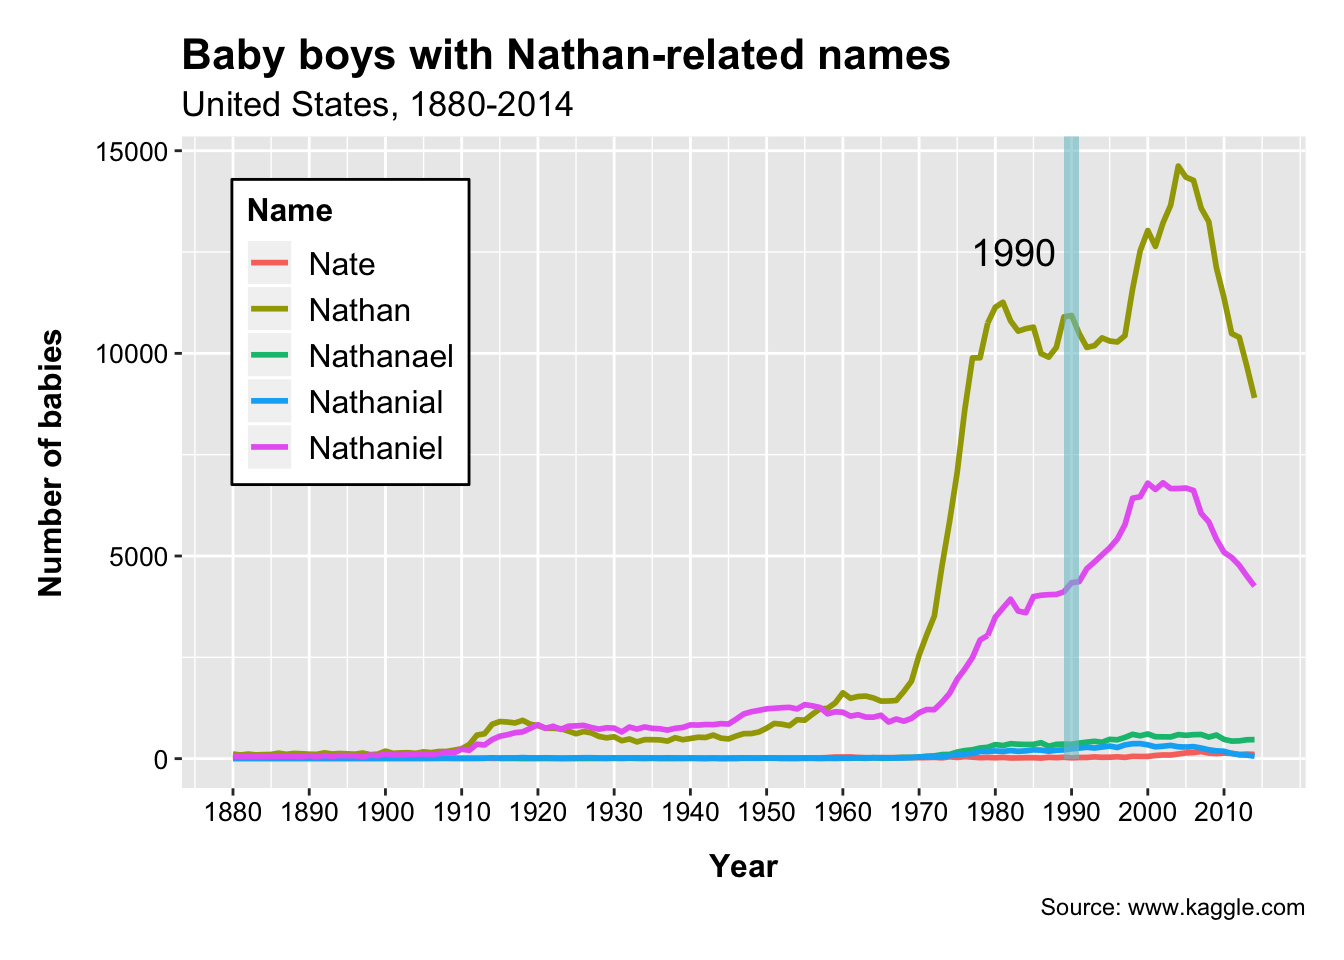
\includegraphics{nathan_plot_files/figure-latex/plot-1.pdf}

\subsubsection{Interactive Plot}\label{interactive-plot}

\begin{Shaded}
\begin{Highlighting}[]
\NormalTok{## interactive plot}
\NormalTok{p2 <-}\StringTok{ }\KeywordTok{ggplot}\NormalTok{(}\DataTypeTok{data=}\NormalTok{dnn, }\KeywordTok{aes}\NormalTok{(}\DataTypeTok{x=}\NormalTok{Year, }\DataTypeTok{y=}\NormalTok{Count, }\DataTypeTok{color=}\NormalTok{Name)) }\OperatorTok{+}\StringTok{ }
\StringTok{  }\KeywordTok{geom_line}\NormalTok{() }\OperatorTok{+}\StringTok{ }
\StringTok{  }\KeywordTok{geom_point}\NormalTok{() }\OperatorTok{+}\StringTok{ }
\StringTok{  }\KeywordTok{ylab}\NormalTok{(}\StringTok{'Number of babies'}\NormalTok{) }\OperatorTok{+}\StringTok{ }
\StringTok{  }\KeywordTok{theme}\NormalTok{(}
    \DataTypeTok{plot.margin =} \KeywordTok{unit}\NormalTok{(}\KeywordTok{c}\NormalTok{(}\DecValTok{1}\NormalTok{,}\DecValTok{1}\NormalTok{,}\DecValTok{1}\NormalTok{,}\DecValTok{1}\NormalTok{), }\StringTok{'lines'}\NormalTok{)}
\NormalTok{  )}

\NormalTok{## in order to make interactive, we will view the plot using ggplotly() function}
\CommentTok{#ggplotly(p2)}
\NormalTok{## you should be able to hover mouse over individual points to see count and year}
\NormalTok{## if you don't want the graph to show up inside R markdown file:}
\NormalTok{    ## click on gear aside of knit at top}
\NormalTok{    ## select 'Chuck Output in Console'}
\end{Highlighting}
\end{Shaded}


\end{document}
